% meta.concepts: 2D force equilibrium
% meta.tags: realistic
% acknowledge: Peter Seiler & Luke Melander graciously shared Spring 2019 course material
% source: 2019 P. Seiler AEM2011 HW 2


The figure below shows a banner hanging on campus along with an idealized diagram for this banner. The banner has length $L = 7.5m$, height $H = 1.5m$, and mass $m = 5kg$. Assume:
\begin{enumerate}
  \item the cables directions are as shown with $\tan(\phi) = \frac{H}{L}$
  \item the tension in cable A is twice that of cable C
  \item the tension in cable B is twice that of cable D
\end{enumerate}
Given these assumptions estimate the tension in each cable so that there is zero net force on the banner.

\begin{figure}[ht!]
  \centering
  \includegraphics[height=1.8in]{figa.png}
  \includegraphics[height=1.8in]{figb.png}
\end{figure}

% \ifthenelse{ \equal{\soln}{true} }{
%   \vspace{.5cm}
%   \rule{\textwidth}{.4pt}
%   \vspace{.5cm}
%   \textbf{Solution:}
%   \begin{figure}[ht!]
%     \centering
%     \includegraphics[width=0.9\textwidth]{soln.png}
%   \end{figure}
% }
